\subsection{Embedded (child) model preparation}

To run an embedded model, the user must provide the grid, the surface 
forcing and the initial conditions. To name the different files,
AGRIF employs a specific strategy: if the parent file names are of
the form: XXX.nc, the first child names will be of the form: 
XXX.nc.1, the second: XXX.nc.2, etc... 
This convention is also applied for the "roms.in" input files.

A graphic user interface (NestGUI) facilitates the generation of 
the different NetCDF files. Launch nestgui in the Matlab session 
(in the $\sim$/Roms\_tools/Run/ directory):
\\ \\
$>>$\\
$>>$ nestgui
\\ \\
A window pops up, asking for a "PARENT GRID" NetCDF file 
(Figure \ref{fig:nestgui3}). In our Benguela test case, you should select 
$\sim$/Roms\_tools/Run/ROMSFILES/roms\_grd.nc (grid file) and click "open".
The main window appears (Figure \ref{fig:nestgui4}).

\begin{figure}[!ht]
\centering
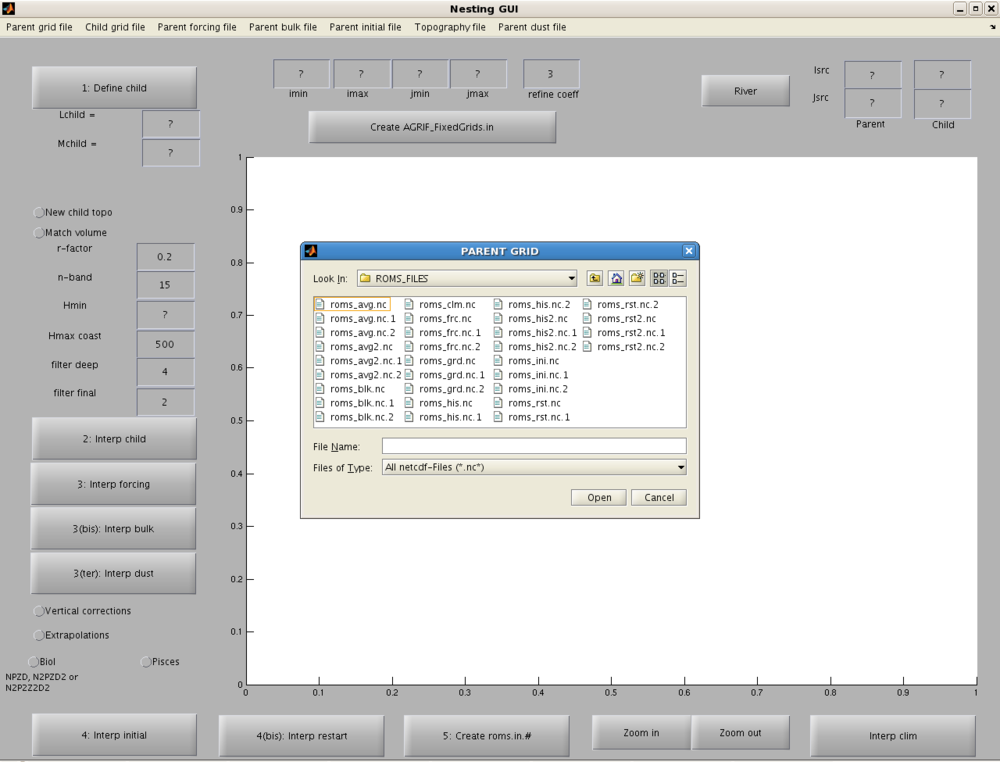
\includegraphics[width=12cm]{Figures/nestgui_entrance.eps}
\caption{Entrance window of NestGUI}
\label{fig:nestgui3}
\end{figure}

\begin{figure}[!ht]
%\centerline{\psfig{figure=nestgui7.eps,width=12cm}}
\centering
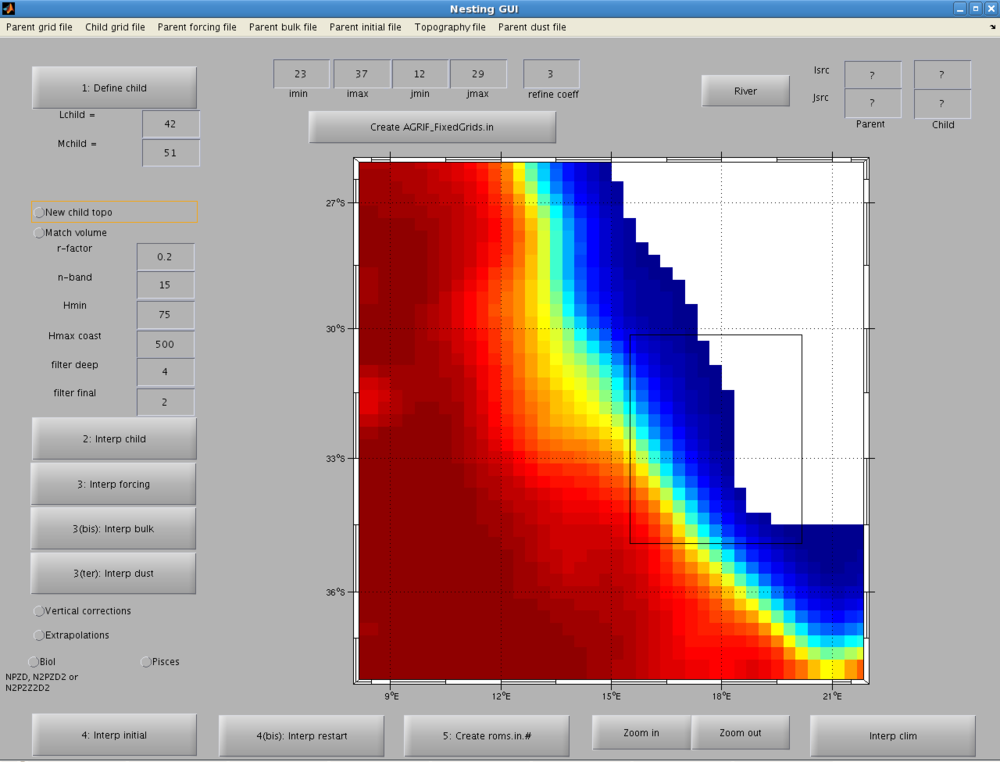
\includegraphics[width=1\textwidth]{Figures/nestgui_vizu.eps}
\caption{The NestGUI main window}
\label{fig:nestgui4}
\end{figure} 

% \begin{figure}[!ht]
% \centerline{\psfig{figure=nesting.eps,width=12cm}}
% \caption{The NestGUI main window}
% \label{fig:nestgui4}
% \end{figure}

To generate the child model you should follow several steps:

\begin{enumerate}

\item To define the child domain, click "Define child" and create the child domain on
  the main window. The size of the grid child (Lchild and Mchild) is now visible.
  This operation can be redone until you are satisfied with the size and the position
  of the child domain. The child domain can be finely tuned using the imin, imax,
  jmin and jmax boxes.  Be aware that the mask interpolation from the parent grid to
  the child grid is not optimal close to corners. Parent/Child boundaries should be
  placed where the mask is showing a straight coastline. A warning will be given
  during the interpolation procedure if this is not the case.

\item "Interp child" : It generates the child grid file. Before, you should select if
  you are using a new topography ("New child topo" button) for the child grid or if
  you are just interpolating the parent topography on the child grid. In the first
  case, you should defines what topography file will be used (e.g.
  $\sim$/Roms\_tools/Topo/etopo2.nc or another dataset).  You should also define if
  you want the volume of the child grid to match the volume of the parent close to
  the parent/child boundaries ("Match volume" button, it should be "on" by default).
  You should also define  the \textbf{'r'} factor \citep{Bec93} for topography smoothing
  ("r-factor", 0.25 is safe) and the number of points to connect the child topography
  to the parent topography ("n-band", it follows the relation
  $h_{new}=\alpha.h_{child} + (1-\alpha).h_{parent}$, where $\alpha$ is going from 0
  to 1 in "n-band" points from the parent/child boundaries).  You should also select
  the child minimum depth ("Hmin", it should be lower or equal to the parent minimum
  depth), the maximum depth at the coast ("Hmax coast"), the number of selective
  hanning filter passes for the deep regions ("n filter deep") and the number of
  final hanning filter passes ("n filter final").

\item "Interp forcing": It interpolates the parent surface forcing on the child grid.
  Select the parent forcing file to be interpolated (e.g.
  $\sim$/Roms\_tools/Run/ROMSFILES/roms\_frc.nc).  The child forcing file
  roms\_frc.nc.1 will be created.  The parent surface fluxes are interpolated on the
  child grid.  You can use "Interp bulk" if you are using a bulk formula.  In this
  case, the parent bulk file (e.g. $\sim$/Roms\_tools/Run/ROMSFILES/roms\_blk.nc)
  will be interpolated on the child grid.

\item "Interp initial": It interpolates parent initial conditions on the child grid.
  Select the parent initial file (e.g.
  $\sim$/Roms\_tools/Run/ROMSFILES/roms\_ini.nc).  The child initial file (e.g.
  $\sim$/Roms\_tools/Run/ROMSFILES/roms\_ini.nc.1) will be created.  If the
  topographies are different between the parent and the child grids, the child
  initial conditions are vertically re-interpolated. In this case you should check if
  the options \textbf{"vertical corrections"} and \textbf{"extrapolations"}
  are selected. \textbf{It is preferable to always use these options.} \\
  If there are parent biological fields in the initial files, they can be processed
  automatically, we have to define the type of biological models: either NPZD-type
  (NChlPZD, N2ChlPZD2 or N2P2Z2D2) then click on the \textit{\textbf{'Biol'}}
  button, either PISCES biogeochemical model, then click on the
  \textit{\textbf{'Pisces'}} button. The fields needed for the initialization of
  these biological model will be processed. \\
  For information, in the case of NPZD type model, there are 4 more fields and in the
  case of PISCES biogeochemical model, there is 8 more fields.

% "Interp biology" can be used to interpolate
% parent biological fields for biogeochemical experiments.

\item "Interp dust": It interpolates parent Iron dust forcing file conditions on the
  child grid.  This is needed only in case of PISCES biogeochemical experiments.
  Select the parent initial file (e.g.
  $\sim$/Roms\_tools/Run/ROMSFILES/roms\_frcbio.nc).  The child initial file (e.g.
  $\sim$/Roms\_tools/Run/ROMSFILES/roms\_frcbio.nc.1) will be created.

\item "Interp restart" generates a child restart file from
  a parent restart file \\
  (e.g. $\sim$/Roms\_tools/Run/ROMSFILES/roms\_rst.nc).  This can be done to "hot
  start" a child model after the spin-up of the parent model. As in the case of
  initial files generation, there is the possibility to compute ans write in the
  nested restart file either the biological fields from NPZD-type biological model,
  either the PISCES biogeochemical fields.  For this purpose, click either on the
  \textit{\textbf{'Biol'}} button, either on the the \textit{\textbf{'Pisces'}}
  button.

\item You can click on "Create roms.in.*" to generate a child input file (roms.in.1)
  from the parent input file and click on "Create AGRIF\_FixedGrids.in" to generate a
  AGRIF\_FixedGrids.in file (the file which defines the child grid position in the
  parent grid).

\item "River" can be used to locate the river on the coast.

\item "Interp clim" can be useful to generate boundary conditions to test the child
  model alone. As in the case of restart an initial nested files generation, during
  the eventual phase of creation of a nested clim file, the fields related to the
  NPZD-type biological models or the PISCES one can be computed and written in the
  nested clim file.  As usual, click either on the \textit{\textbf{'Biol'}} button or
  on the \textit{\textbf{'Pisces'}} button.




\end{enumerate}
\subsection{Compiling and running the model}
The ROMS nesting procedure needs a Fortran 95 compiler. For Linux PCs,
the Intel Fortran Compiler (ifort) is available at \\
http://www.intel.com/software/products/compilers/flin/noncom.htm.  To be able to
compile ROMS with ifort, you should change the corresponding
comments in jobcomp. \\

To activate the AGRIF nesting procedure, define AGRIF in
$\sim$/Roms\_tools/Run/cppdefs.h. Moreover, to activate the AGRIF nesting with the
$2$-way capability, define AGRIF and AGRIF\_$2$WAYS. \\




It is possible to edit the file AGRIF\_FixedGrids.in.  This file contains the child
grid positions (i.e. imin,imax,jmin,jmax) and coefficients of refinement. A first
line gives the number of children grids per parent (if AGRIF\_STORE\_BAROT\_CHILD is
defined, only one child grid can be defined per parent grid). A second line gives the
relative position of each grid and the coefficient of refinement for each dimension.
Edit the input files roms.in.1, roms.in.2 , etc... to define correctly the file names
and the time steps. To run the model, simply type at the prompt: roms roms.in. \\

To visualize the ROMS model outputs for different grid levels, 
change the value in the "child models" box
in roms\_gui.


